\begin{frame}
    \myheading{Module 7.2: Link between PCA and Autoencoders}
\end{frame}



\begin{frame}
    \begin{columns}
        \column{0.5\textwidth}
        %\vspace{1cm}
        \begin{overlayarea}{\textwidth}{\textheight}
            \tikzstyle{input_neuron}=[circle,draw=red!50,fill=red!10,thick,minimum size=6mm]
\tikzstyle{hidden_neuron}=[circle,draw=blue!50,fill=cyan!10,thick,minimum size=6mm]
\tikzstyle{output_neuron}=[circle,draw=green!50,fill=green!10,thick,minimum size=6mm]

\tikzstyle{input}=[circle,draw=black!50,fill=black!20,thick,minimum size=6mm]

\begin{center}
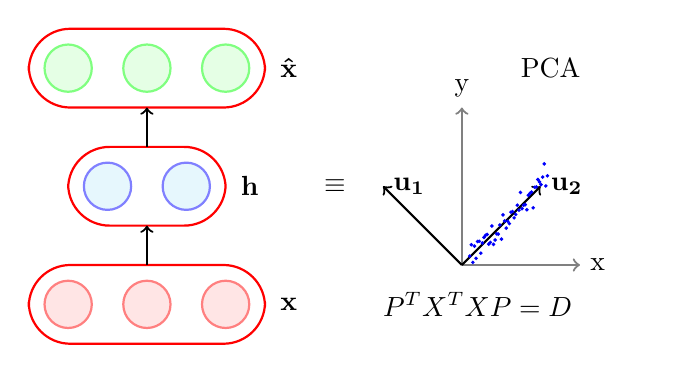
\begin{tikzpicture}


\node [input_neuron] (neuron01) at (6.5,4.5) {};
\node [input_neuron] (neuron02) at (7.5,4.5){};
\node [input_neuron] (neuron03) at (8.5,4.5) {};
%\node [input_neuron] (neuron04) at (9.5,4.5) {};
%\node [input_neuron] (neuron05) at (10.5,4.5) {};
\node [hidden_neuron] (neuron51) at (7,6) {} ;
\node [hidden_neuron] (neuron52) at (8,6)  {};
%\node [hidden_neuron] (neuron53) at (9,6)  {};
%\node [hidden_neuron] (neuron54) at (10,6)  {};

\node [output_neuron] (neuron11) at (6.5,7.5)  {};
\node [output_neuron] (neuron12) at (7.5,7.5)  {};
\node [output_neuron] (neuron13) at (8.5,7.5)  {};
%\node [output_neuron] (neuron14) at (9.5,7.5)  {};
%\node [output_neuron] (neuron15) at (10.5,7.5)  {};

\node[text width=0.01cm] at (9.2,4.5) {$\mathbf{x}$};
\node[text width=0.01cm] at (8.7,6) {$\mathbf{h}$};
\node[text width=0.01cm] at (9.2,7.5) {$\mathbf{\hat{x}}$};

\draw[red!100,thick,solid,rounded corners=15pt] (6,4) rectangle (9,5);
\draw[red!100,thick,solid,rounded corners=15pt] (6.5,5.5) rectangle (8.5,6.5);
\draw[red!100,thick,solid,rounded corners=15pt] (6,7) rectangle (9,8);


\draw[thick,->] (7.5,5) -- (7.5,5.5);

\draw[thick,->] (7.5,6.5) -- (7.5,7);


\node[text width=0.5cm] at (10,6) {$\equiv$};
  \node[text width=1.5cm] at (13,7.5) {PCA};
  \node[text width=3cm] at (12,4.5) {$P^TX^TXP=D$};
    \draw [thick, gray, ->] (11.5,5) -- (11.5,7)      % draw y-axis line
        node [above, black] {y};              % add label for y-axis
        %node [below,black]{$-y$};
    \draw [thick, gray, ->] (11.5,5) -- (13,5)      % draw x-axis line
        node [right, black] {x};  
    \draw [thick, black, ->] (11.5,5) -- (10.5,6)      % draw u1 line
        node [right, black] {$\mathbf{u_1}$}; 
    \draw [thick, black, ->] (11.5,5) -- (12.5,6)      % draw u2 line
        node [right, black] {$\mathbf{u_2}$}; 

%\if 1
\foreach \x/\y in {0.5/0.511870677093,0.520134228188/0.657474112041,0.540268456376/0.433301054831,0.560402684564/0.639402738784,0.580536912752/0.484888418032,0.60067114094/0.698401610126,0.620805369128/0.7012649978,0.640939597315/0.550258599782,0.661073825503/0.678863257247,0.681208053691/0.75063942818,0.701342281879/0.776722844493,0.721476510067/0.787974629261,0.741610738255/0.664867942136,0.761744966443/0.686496368534,0.781879194631/0.895235993285,0.802013422819/0.661601738133,0.822147651007/0.717376222072,0.842281879195/0.796219038444,0.862416107383/0.792290066926,0.88255033557/0.908555964509,0.902684563758/0.728213610997,0.922818791946/1.03682525621,0.942953020134/0.959254604949,0.963087248322/0.868395203865,0.98322147651/0.954903379431,1.0033557047/0.925500701421,1.02348993289/1.0700072327,1.04362416107/1.07910784654,1.06375838926/0.998680883498,1.08389261745/1.04215184899,1.10402684564/1.15961695354,1.12416107383/1.09641078989,1.14429530201/1.32135817413,1.1644295302/1.11554678055,1.18456375839/1.15881333579,1.20469798658/1.16650720076,1.22483221477/1.10170000196,1.24496644295/1.2856802819,1.26510067114/1.31032588214,1.28523489933/1.32664087434,1.30536912752/1.12586374789,1.3255033557/1.38744778116,1.34563758389/1.39149477354,1.36577181208/1.4858410387,1.38590604027/1.45489220706,1.40604026846/1.42066727608,1.42617449664/1.51638552543,1.44630872483/1.68453235672,1.46644295302/1.40404774902,1.48657718121/1.53217972768} 
                {
                \node at (11.1+\x,4.6+\y)[circle,draw=blue,fill=black,inner sep=0pt,minimum size=0.3mm]{};
                }
%\fi 
\end{tikzpicture} 
\end{center}

        \end{overlayarea}

        \column{0.5\textwidth}
        \begin{overlayarea}{\textwidth}{\textheight}
            \begin{itemize}\justifying
                \item We will now see that the encoder part of an autoencoder is equivalent to PCA if we
                \begin{itemize}\justifying
                    \item<2-> use a linear encoder
                    \item<3-> use a linear decoder
                    \item<4-> use squared error loss function
                    \item<5-> normalize the inputs to 
                    \begin{align*}
                         \hat{x}_{ij} = \frac{1}{\sqrt{m}}\Bigg(x_{ij}-\frac{1}{m}\sum\limits_{k=1}^mx_{kj}\Bigg) 
                    \end{align*}
                \end{itemize}
            \end{itemize}
        \end{overlayarea}
    \end{columns}
\end{frame}


\begin{frame}
    %\vspace{0.1in}
    \begin{columns}
        \column{0.5\textwidth}
        \begin{overlayarea}{\textwidth}{\textheight}
            \tikzstyle{input_neuron}=[circle,draw=red!50,fill=red!10,thick,minimum size=6mm]
\tikzstyle{hidden_neuron}=[circle,draw=blue!50,fill=cyan!10,thick,minimum size=6mm]
\tikzstyle{output_neuron}=[circle,draw=green!50,fill=green!10,thick,minimum size=6mm]

\tikzstyle{input}=[circle,draw=black!50,fill=black!20,thick,minimum size=6mm]

\begin{center}
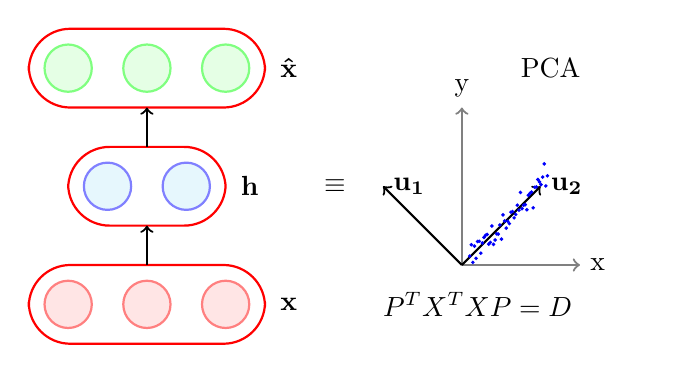
\begin{tikzpicture}


\node [input_neuron] (neuron01) at (6.5,4.5) {};
\node [input_neuron] (neuron02) at (7.5,4.5){};
\node [input_neuron] (neuron03) at (8.5,4.5) {};
%\node [input_neuron] (neuron04) at (9.5,4.5) {};
%\node [input_neuron] (neuron05) at (10.5,4.5) {};
\node [hidden_neuron] (neuron51) at (7,6) {} ;
\node [hidden_neuron] (neuron52) at (8,6)  {};
%\node [hidden_neuron] (neuron53) at (9,6)  {};
%\node [hidden_neuron] (neuron54) at (10,6)  {};

\node [output_neuron] (neuron11) at (6.5,7.5)  {};
\node [output_neuron] (neuron12) at (7.5,7.5)  {};
\node [output_neuron] (neuron13) at (8.5,7.5)  {};
%\node [output_neuron] (neuron14) at (9.5,7.5)  {};
%\node [output_neuron] (neuron15) at (10.5,7.5)  {};

\node[text width=0.01cm] at (9.2,4.5) {$\mathbf{x}$};
\node[text width=0.01cm] at (8.7,6) {$\mathbf{h}$};
\node[text width=0.01cm] at (9.2,7.5) {$\mathbf{\hat{x}}$};

\draw[red!100,thick,solid,rounded corners=15pt] (6,4) rectangle (9,5);
\draw[red!100,thick,solid,rounded corners=15pt] (6.5,5.5) rectangle (8.5,6.5);
\draw[red!100,thick,solid,rounded corners=15pt] (6,7) rectangle (9,8);


\draw[thick,->] (7.5,5) -- (7.5,5.5);

\draw[thick,->] (7.5,6.5) -- (7.5,7);


\node[text width=0.5cm] at (10,6) {$\equiv$};
  \node[text width=1.5cm] at (13,7.5) {PCA};
  \node[text width=3cm] at (12,4.5) {$P^TX^TXP=D$};
    \draw [thick, gray, ->] (11.5,5) -- (11.5,7)      % draw y-axis line
        node [above, black] {y};              % add label for y-axis
        %node [below,black]{$-y$};
    \draw [thick, gray, ->] (11.5,5) -- (13,5)      % draw x-axis line
        node [right, black] {x};  
    \draw [thick, black, ->] (11.5,5) -- (10.5,6)      % draw u1 line
        node [right, black] {$\mathbf{u_1}$}; 
    \draw [thick, black, ->] (11.5,5) -- (12.5,6)      % draw u2 line
        node [right, black] {$\mathbf{u_2}$}; 

%\if 1
\foreach \x/\y in {0.5/0.511870677093,0.520134228188/0.657474112041,0.540268456376/0.433301054831,0.560402684564/0.639402738784,0.580536912752/0.484888418032,0.60067114094/0.698401610126,0.620805369128/0.7012649978,0.640939597315/0.550258599782,0.661073825503/0.678863257247,0.681208053691/0.75063942818,0.701342281879/0.776722844493,0.721476510067/0.787974629261,0.741610738255/0.664867942136,0.761744966443/0.686496368534,0.781879194631/0.895235993285,0.802013422819/0.661601738133,0.822147651007/0.717376222072,0.842281879195/0.796219038444,0.862416107383/0.792290066926,0.88255033557/0.908555964509,0.902684563758/0.728213610997,0.922818791946/1.03682525621,0.942953020134/0.959254604949,0.963087248322/0.868395203865,0.98322147651/0.954903379431,1.0033557047/0.925500701421,1.02348993289/1.0700072327,1.04362416107/1.07910784654,1.06375838926/0.998680883498,1.08389261745/1.04215184899,1.10402684564/1.15961695354,1.12416107383/1.09641078989,1.14429530201/1.32135817413,1.1644295302/1.11554678055,1.18456375839/1.15881333579,1.20469798658/1.16650720076,1.22483221477/1.10170000196,1.24496644295/1.2856802819,1.26510067114/1.31032588214,1.28523489933/1.32664087434,1.30536912752/1.12586374789,1.3255033557/1.38744778116,1.34563758389/1.39149477354,1.36577181208/1.4858410387,1.38590604027/1.45489220706,1.40604026846/1.42066727608,1.42617449664/1.51638552543,1.44630872483/1.68453235672,1.46644295302/1.40404774902,1.48657718121/1.53217972768} 
                {
                \node at (11.1+\x,4.6+\y)[circle,draw=blue,fill=black,inner sep=0pt,minimum size=0.3mm]{};
                }
%\fi 
\end{tikzpicture} 
\end{center}

        \end{overlayarea}

        \column{0.5\textwidth}
        \begin{overlayarea}{\textwidth}{\textheight}
            \begin{itemize}\justifying
                \item<1-> First let us consider the implication of normalizing the inputs to
                \begin{align*}
                    \hat{x}_{ij} = \frac{1}{\sqrt{m}}\Bigg(x_{ij}-\frac{1}{m}\sum\limits_{k=1}^mx_{kj}\Bigg) 
                \end{align*}
                \vspace{-0.2in}
                
                \item<2-> The operation in the bracket ensures that the data now has 0 mean along each dimension $j$ (we are subtracting the mean)
                \item<3-> Let $X^{'}$ be this zero mean data matrix then what the above normalization gives us is $X= \frac{1}{\sqrt{m}}X^{'}$
                \item<4-> Now $(X)^TX =\frac{1}{m}(X')^TX'$ is the covariance matrix (recall that covariance matrix plays an important role in PCA)
            \end{itemize}
        \end{overlayarea}
    \end{columns}
\end{frame}


\begin{frame}
    \begin{columns}
        \column{0.5\textwidth}
        \begin{overlayarea}{\textwidth}{\textheight}
            \tikzstyle{input_neuron}=[circle,draw=red!50,fill=red!10,thick,minimum size=6mm]
\tikzstyle{hidden_neuron}=[circle,draw=blue!50,fill=cyan!10,thick,minimum size=6mm]
\tikzstyle{output_neuron}=[circle,draw=green!50,fill=green!10,thick,minimum size=6mm]

\tikzstyle{input}=[circle,draw=black!50,fill=black!20,thick,minimum size=6mm]

\begin{center}
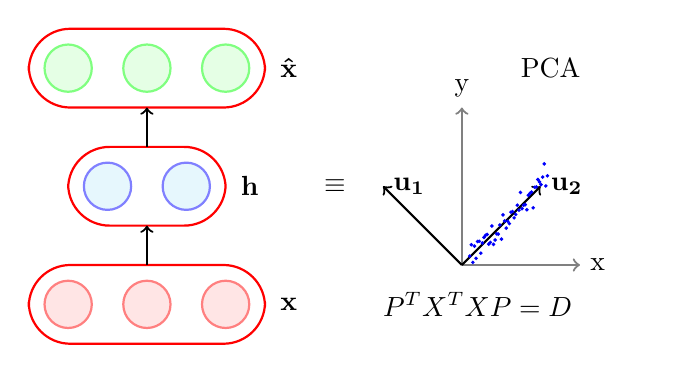
\begin{tikzpicture}


\node [input_neuron] (neuron01) at (6.5,4.5) {};
\node [input_neuron] (neuron02) at (7.5,4.5){};
\node [input_neuron] (neuron03) at (8.5,4.5) {};
%\node [input_neuron] (neuron04) at (9.5,4.5) {};
%\node [input_neuron] (neuron05) at (10.5,4.5) {};
\node [hidden_neuron] (neuron51) at (7,6) {} ;
\node [hidden_neuron] (neuron52) at (8,6)  {};
%\node [hidden_neuron] (neuron53) at (9,6)  {};
%\node [hidden_neuron] (neuron54) at (10,6)  {};

\node [output_neuron] (neuron11) at (6.5,7.5)  {};
\node [output_neuron] (neuron12) at (7.5,7.5)  {};
\node [output_neuron] (neuron13) at (8.5,7.5)  {};
%\node [output_neuron] (neuron14) at (9.5,7.5)  {};
%\node [output_neuron] (neuron15) at (10.5,7.5)  {};

\node[text width=0.01cm] at (9.2,4.5) {$\mathbf{x}$};
\node[text width=0.01cm] at (8.7,6) {$\mathbf{h}$};
\node[text width=0.01cm] at (9.2,7.5) {$\mathbf{\hat{x}}$};

\draw[red!100,thick,solid,rounded corners=15pt] (6,4) rectangle (9,5);
\draw[red!100,thick,solid,rounded corners=15pt] (6.5,5.5) rectangle (8.5,6.5);
\draw[red!100,thick,solid,rounded corners=15pt] (6,7) rectangle (9,8);


\draw[thick,->] (7.5,5) -- (7.5,5.5);

\draw[thick,->] (7.5,6.5) -- (7.5,7);


\node[text width=0.5cm] at (10,6) {$\equiv$};
  \node[text width=1.5cm] at (13,7.5) {PCA};
  \node[text width=3cm] at (12,4.5) {$P^TX^TXP=D$};
    \draw [thick, gray, ->] (11.5,5) -- (11.5,7)      % draw y-axis line
        node [above, black] {y};              % add label for y-axis
        %node [below,black]{$-y$};
    \draw [thick, gray, ->] (11.5,5) -- (13,5)      % draw x-axis line
        node [right, black] {x};  
    \draw [thick, black, ->] (11.5,5) -- (10.5,6)      % draw u1 line
        node [right, black] {$\mathbf{u_1}$}; 
    \draw [thick, black, ->] (11.5,5) -- (12.5,6)      % draw u2 line
        node [right, black] {$\mathbf{u_2}$}; 

%\if 1
\foreach \x/\y in {0.5/0.511870677093,0.520134228188/0.657474112041,0.540268456376/0.433301054831,0.560402684564/0.639402738784,0.580536912752/0.484888418032,0.60067114094/0.698401610126,0.620805369128/0.7012649978,0.640939597315/0.550258599782,0.661073825503/0.678863257247,0.681208053691/0.75063942818,0.701342281879/0.776722844493,0.721476510067/0.787974629261,0.741610738255/0.664867942136,0.761744966443/0.686496368534,0.781879194631/0.895235993285,0.802013422819/0.661601738133,0.822147651007/0.717376222072,0.842281879195/0.796219038444,0.862416107383/0.792290066926,0.88255033557/0.908555964509,0.902684563758/0.728213610997,0.922818791946/1.03682525621,0.942953020134/0.959254604949,0.963087248322/0.868395203865,0.98322147651/0.954903379431,1.0033557047/0.925500701421,1.02348993289/1.0700072327,1.04362416107/1.07910784654,1.06375838926/0.998680883498,1.08389261745/1.04215184899,1.10402684564/1.15961695354,1.12416107383/1.09641078989,1.14429530201/1.32135817413,1.1644295302/1.11554678055,1.18456375839/1.15881333579,1.20469798658/1.16650720076,1.22483221477/1.10170000196,1.24496644295/1.2856802819,1.26510067114/1.31032588214,1.28523489933/1.32664087434,1.30536912752/1.12586374789,1.3255033557/1.38744778116,1.34563758389/1.39149477354,1.36577181208/1.4858410387,1.38590604027/1.45489220706,1.40604026846/1.42066727608,1.42617449664/1.51638552543,1.44630872483/1.68453235672,1.46644295302/1.40404774902,1.48657718121/1.53217972768} 
                {
                \node at (11.1+\x,4.6+\y)[circle,draw=blue,fill=black,inner sep=0pt,minimum size=0.3mm]{};
                }
%\fi 
\end{tikzpicture} 
\end{center}

        \end{overlayarea}


        \column{0.5\textwidth}
        \begin{overlayarea}{\textwidth}{\textheight}
            \begin{itemize}\justifying
                \item<2-> First we will show that if we use linear decoder and a squared error loss function then
                \item<3->The optimal solution to the following objective function 
                    \begin{align*}
                      \onslide<4-> {\frac{1}{m}\sum\limits_{i=1}^{m}\sum\limits_{j=1}^n(x_{ij}-\hat{x}_{ij})^2}
                    \end{align*}
                    \onslide<5->{is obtained when we use a linear encoder.}
            \end{itemize}
        \end{overlayarea}
    \end{columns}
\end{frame}


\begin{frame}
    \begin{overlayarea}{\textwidth}{\textheight}
        \small{
        \begin{equation} \label{equ:1}
            \min\limits_\theta\sum\limits_{i=1}^m\sum\limits_{j=1}^n(x_{ij}-\hat{x}_{ij})^2    
        \end{equation}
        \vspace{-0.1in}

        \begin{itemize}\justifying
            \vspace{-0.2in}
            \item <2-> This is equivalent to 
            \vspace{-0.2in}
            \begin{align*}
                \onslide<3->{\min\limits_{W^*H}(\|X-HW^*\|_F)^2 \hspace{0.2in} \hspace{0.5in}} 
                \onslide<4->{\|A\|_F = \sqrt{\sum\limits_{i=1}^m\sum\limits_{j=1}^na_{ij}^2}}
            \end{align*}
        
            \onslide<5->{(just writing the expression (\ref{equ:1}) in matrix form and using the definition of $||A||_F$) (we are ignoring the biases)}

            \item<6->From SVD we know that optimal solution to the above problem is given by 
            \begin{align*}
                HW^* = U_{.\hspace{0.01in},\leq k}\Sigma_{k,k}V_{.\hspace{0.01in},\leq k}^T
            \end{align*}
        
            \item<7-> By matching variables one possible solution is
            \begin{align*}
                H &=U_{.\hspace{0.01in},\leq k}\Sigma_{k,k} \\
                W^* &= V_{.\hspace{0.01in},\leq k}^T
            \end{align*} 
        \end{itemize}}
    \end{overlayarea}
\end{frame}


\begin{frame}
    \small
    \begin{overlayarea}{\textwidth}{\textheight}
        \vspace{5pt}
        We will now show that $H$ is a linear encoding and find an expression for the encoder weights $W$
        \begin{align*}
            \onslide<2->{H  &= U_{.\hspace{0.01in},\leq k}\Sigma_{k,k}\\}
            \onslide<3->{      &= (XX^T)(XX^T)^{-1}U_{.\hspace{0.01in}, \leq K}\Sigma_{k,k} &\quad \textit{(pre-multiplying $(XX^T)(XX^T)^{-1} = I$)} \\}
            \onslide<4->{      &= (XV\Sigma^TU^T)(U\Sigma V^TV\Sigma^TU^T)^{-1}U_{.\hspace{0.01in},\leq k}\Sigma_{k,k} &\quad \textit{(using $X=U\Sigma V^T$)} \\}
            \onslide<5->{      &= XV\Sigma^TU^T(U\Sigma\Sigma^TU^T)^{-1}U_{.\hspace{0.01in}, \leq k}\Sigma_{k,k} &\quad (V^TV = I)\\} 
            \onslide<6->{      &= XV\Sigma^TU^TU(\Sigma\Sigma^T)^{-1}U^TU_{.\hspace{0.01in}, \leq k}\Sigma_{k,k} &\quad ((ABC)^{-1} = C^{-1}B^{-1}A^{-1})\\}
            \onslide<7->{      &= XV\Sigma^T(\Sigma\Sigma^T)^{-1}U^TU_{.\hspace{0.01in}, \leq k}\Sigma_{k,k} &\quad (U^TU = I)\\}
            \onslide<8->{      &= XV\Sigma^T\Sigma^{T^{-1}}\Sigma^{-1}U^TU_{.\hspace{0.01in}, \leq k}\Sigma_{k,k} &\quad ((AB)^{-1} = B^{-1}A^{-1})\\}
            \onslide<9->{      &= XV\Sigma^{-1}I_{.\hspace{0.01in}, \leq k}\Sigma_{k,k} &\quad (U^TU_{.\hspace{0.01in}, \leq k} = I_{.\hspace{0.01in}, \leq k})\\}
            \onslide<10->{     &=XVI_{.\hspace{0.01in}, \leq k} &\quad (\Sigma^{-1}I_{.\hspace{0.01in}, \leq k}=\Sigma_{k,k}^{-1})\\}
            \onslide<11->{H &=XV_{.\hspace{0.01in},\leq k}}
        \end{align*}
        \only<12->{Thus $H$ is a linear transformation of $X$ and $W=V_{.\hspace{0.01in},\leq k}$}
    \end{overlayarea}
\end{frame}


\begin{frame}
    \begin{overlayarea}{\textwidth}{\textheight}
        \begin{itemize}\justifying
            \item<1-> We have encoder $W=V_{.\hspace{0.01in},\leq k}$
            \item<2-> From SVD, we know that $V$ is the matrix of eigen vectors of $X^TX$
            \item<3-> From PCA, we know that $P$ is the matrix of the eigen vectors of the covariance matrix
            \item<4-> We saw earlier that, if entries of $X$ are normalized by
        \end{itemize}
        \only<5->
        {
            \begin{align*}
                         \hat{x}_{ij} = \frac{1}{\sqrt{m}}\Bigg(x_{ij}-\frac{1}{m}\sum\limits_{k=1}^mx_{kj}\Bigg) 
            \end{align*}
            
        }
        \only<6->
        {
            then $X^TX$ is indeed the covariance matrix
        }
        \begin{itemize}
            \item<7-> Thus, the encoder matrix for linear autoencoder($W$) and the projection matrix($P$) for PCA could indeed be the same. Hence proved
        \end{itemize}
    \end{overlayarea}
\end{frame}

\begin{frame}

    \begin{block}{Remember}
        The encoder of a linear autoencoder is equivalent to PCA if we 
        \begin{itemize}\justifying
            \item<2-> use a linear encoder
            \item<3-> use a linear decoder
            \item<4-> use a squared error loss function
            \item<5-> and normalize the inputs to 
        \end{itemize}
        \onslide<6->
        {
            \begin{align*}
                         \hat{x}_{ij} = \frac{1}{\sqrt{m}}\Bigg(x_{ij}-\frac{1}{m}\sum\limits_{k=1}^mx_{kj}\Bigg) 
            \end{align*}            
        }
    \end{block}
\end{frame}
